\section{符号约定}
该手册对数据结构格式,指令的符号表示以及十六进制和二进制数使用的表示方法如下所述。
\subsection{比特和字节顺序}
在存储器中的数据结构的图示中,较小的地址出现在图的底部;地址增加到顶部。比特位置从右到左编号。一个特定比特的数值等于 2 的比特位置次方。英特尔 64 和 IA-32 处理器是“小端”机器;这意味着字的字节从最低有效字节开始编号。见 \autoref{fig:1-1}。
\begin{figure}[H]
\centering
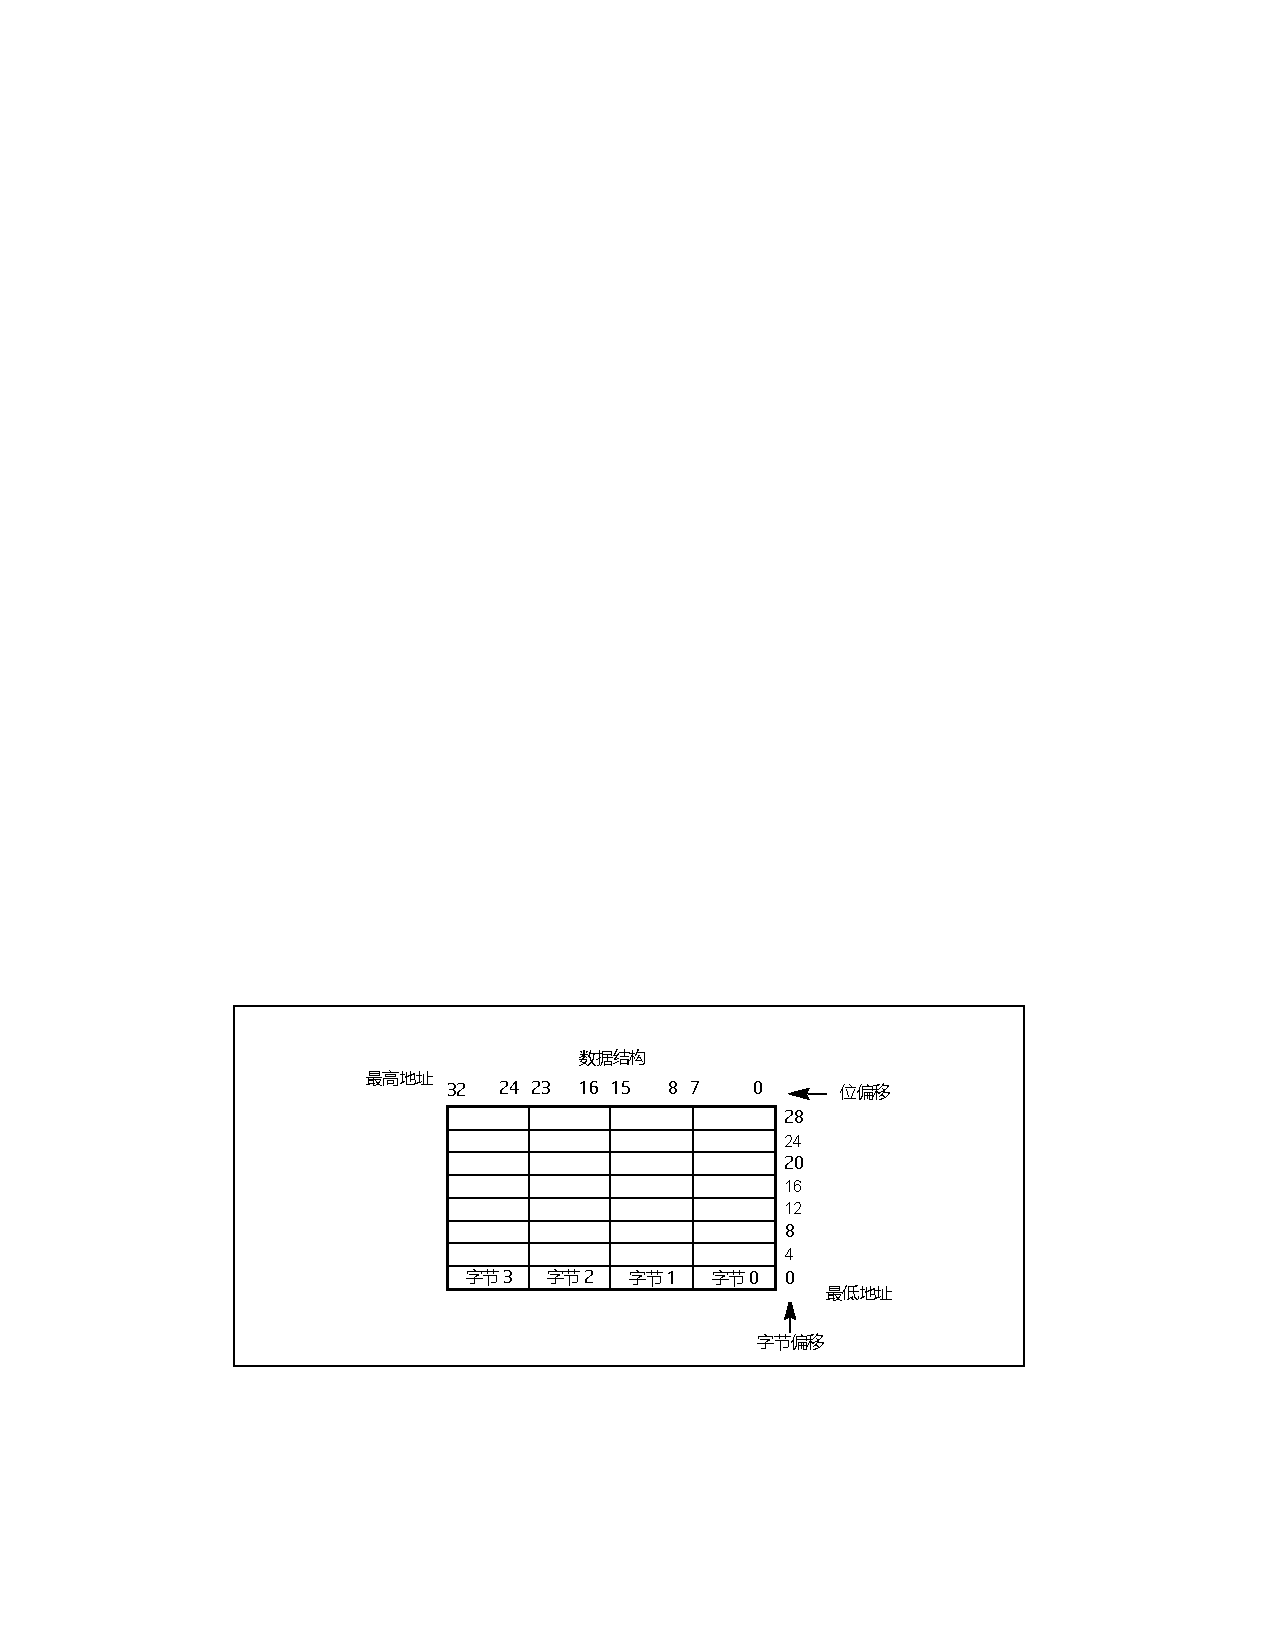
\includegraphics[scale=1]{1-1.pdf}
\caption{位和字节顺序}
\label{fig:1-1}
\end{figure}

\subsection{保留位和软件兼容性}
在许多寄存器和内存分布描述中,一些特定的位被标记为\textbf{保留位}。当某些位被标记为保留位时,软件需要认为这些位将在未来发挥作用(虽然是未知的作用),这对兼容未来处理器来说十分重要。这些保留位的行为是未定义的且不可预测的。

软件在处理保留位时应该遵循以下准则:
\begin{itemize}
	\item 当测试包含保留位的寄存器的值时,不要依赖任何保留位的状态。在测试前标出这些保留位。
	\item 当写入内存或寄存器时不要依赖任何保留位的状态。
	\item 当把信息写入保留位时,不要期望保留位有能力保持信息
	\item 加载寄存器时,始终使用文档中指示的值(如果有的话)加载保留位,或者使用先前从该寄存器读取的保留位的值加载这些保留位。
\end{itemize}

\begin{center}
{\Large \intelblue{\textbf{说明}}}
\end{center}

要避免任何软件依赖于英特尔 64 和 IA-32 寄存器的保留位。

依赖于寄存器中保留位的值将使软件依赖于处理器处理这些位的不确定的方式。

程序依赖于保留位的值将带来与未来处理器不兼容的风险。

\subsubsection{指令的操作数}
所有符号代表的指令都是 IA-32 汇编语言的子集,一个指令有如下格式:

\KAI{标记: 助记符~~参数1, 参数2, 参数3}